% Appendix figures. Paths are relative to HW1/; adjust \graphicspath as needed.

\begin{figure}[htbp]
\centering
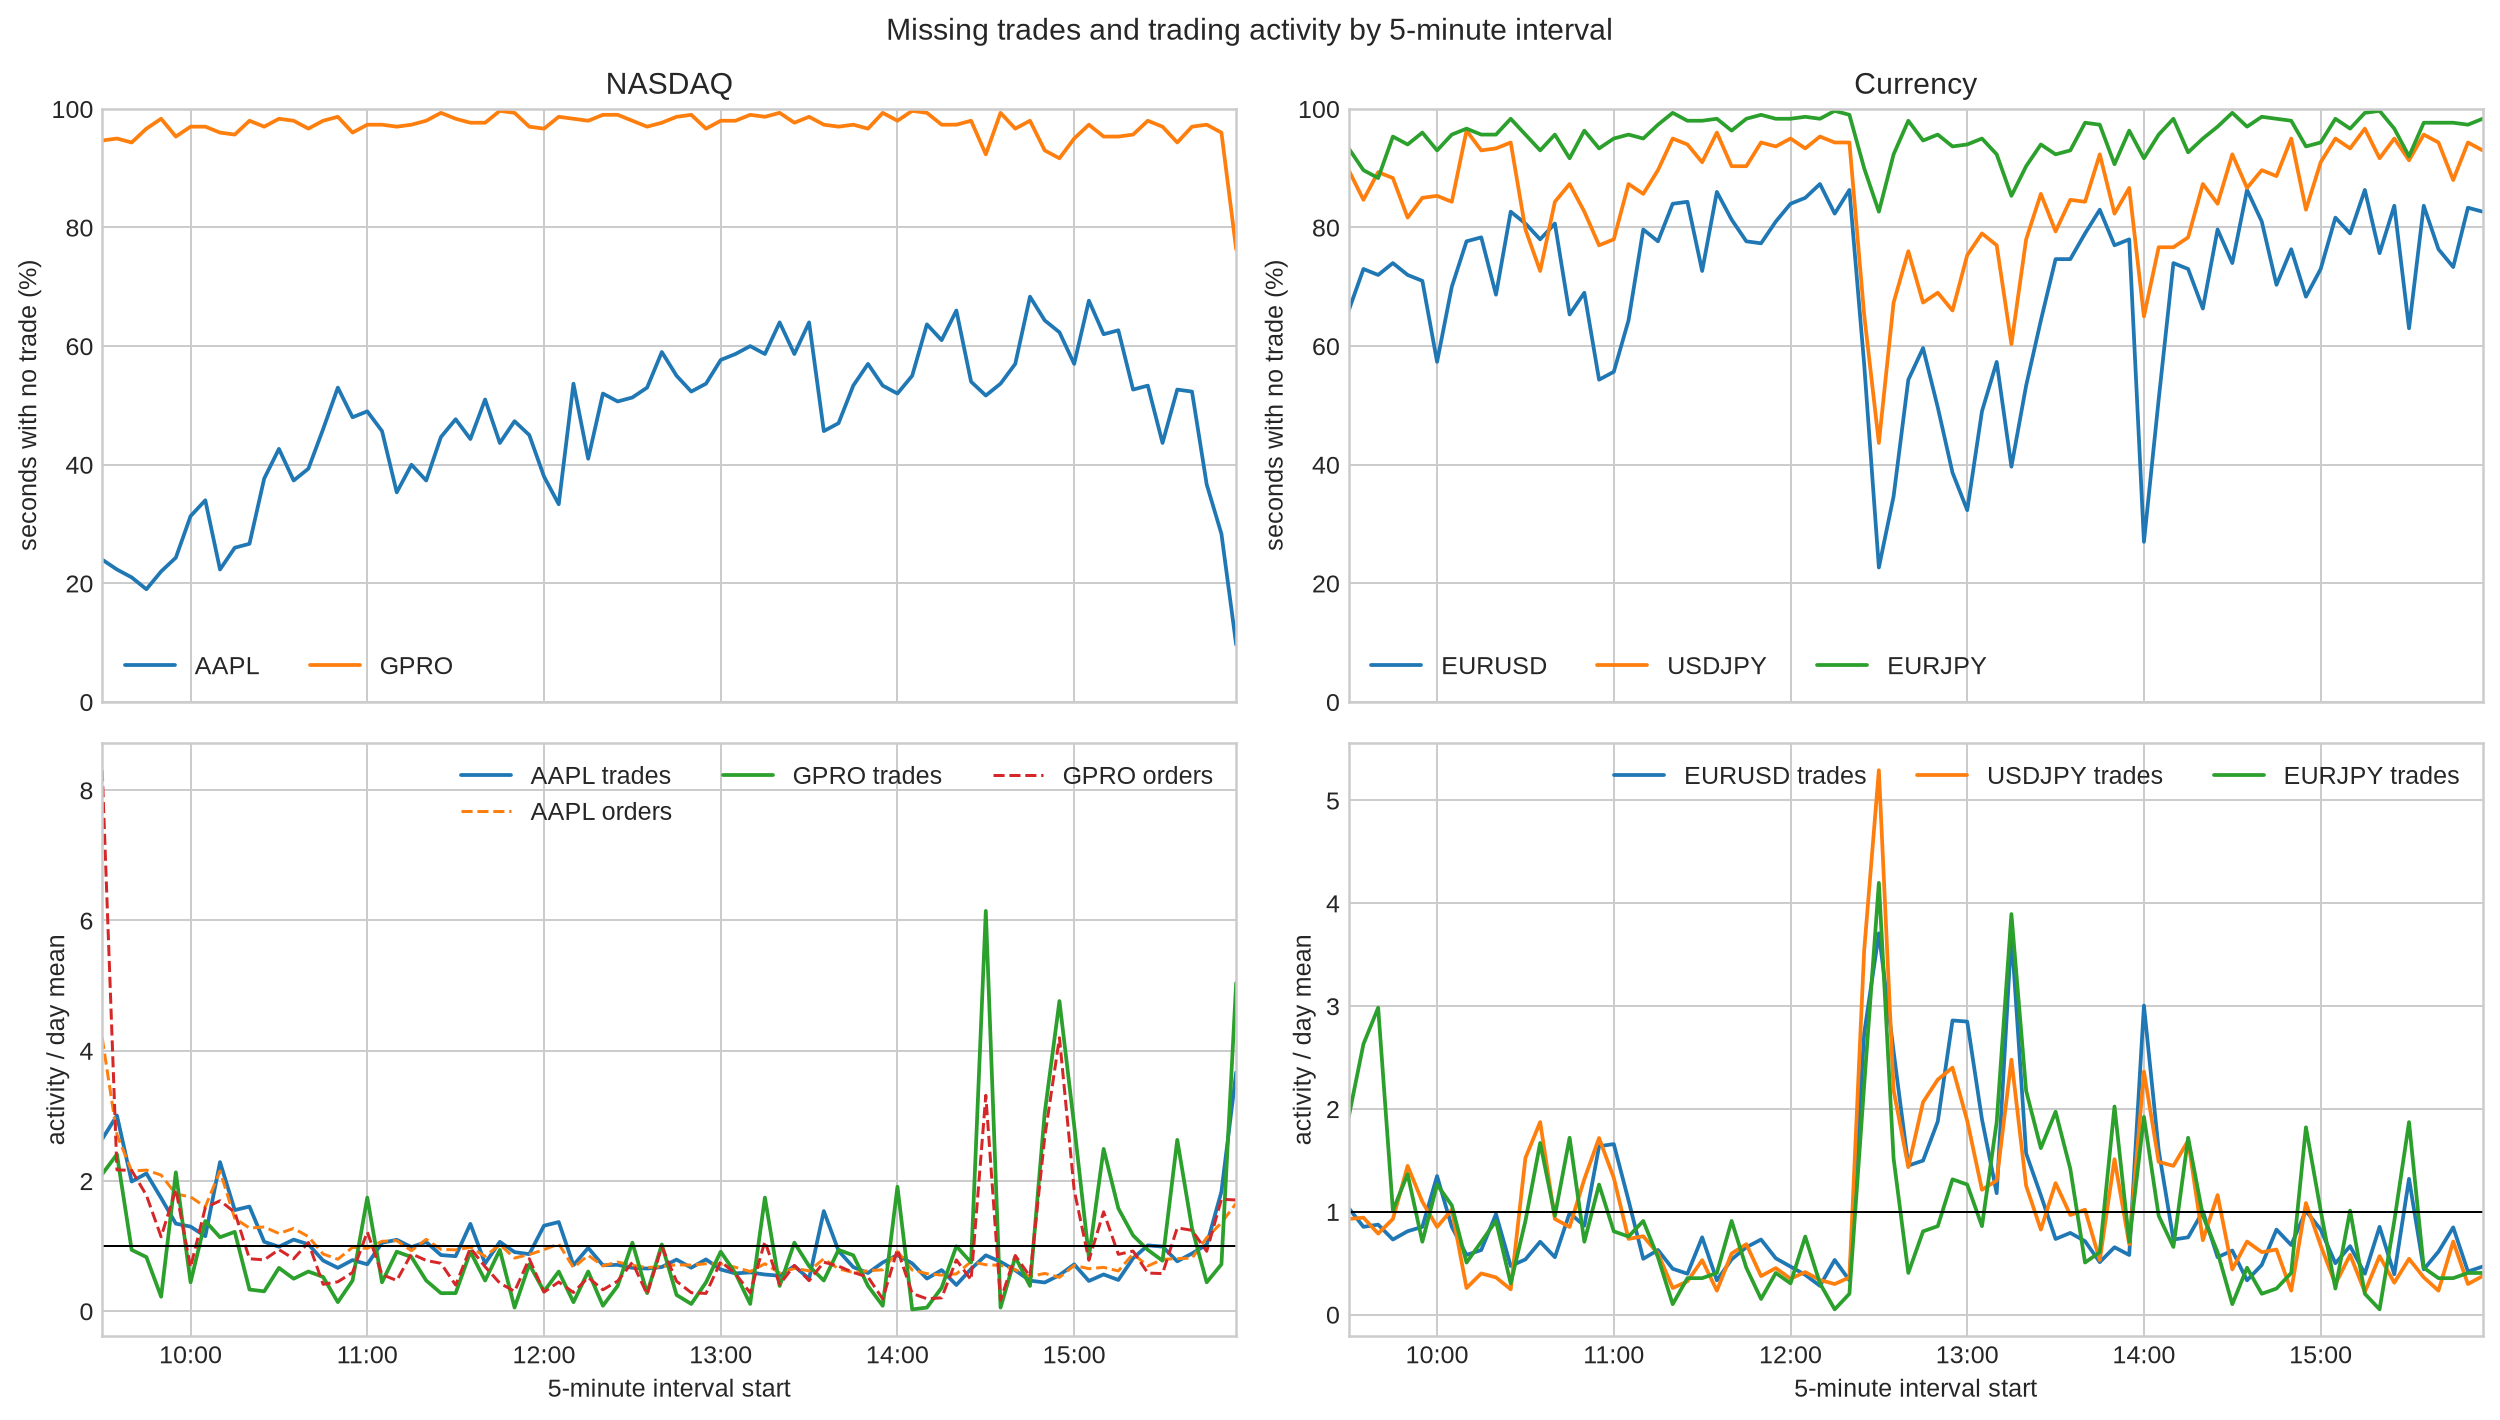
\includegraphics[width=\linewidth]{outputs/figures/A1_missing_trades_activity_5min.png}
\caption{Missing trades and trading activity by five-minute interval. The upper panels show the share of one-second bars in each interval with no transaction. The lower panels show the number of trades (solid) and, for NASDAQ, new displayed orders (dashed) per interval, each divided by its session mean, so that 1.0 is an average interval. NASDAQ is 30 December 2019; currencies are 25 January 2012.}
\label{fig:missing_trades_activity}
\end{figure}

\begin{figure}[htbp]
\centering
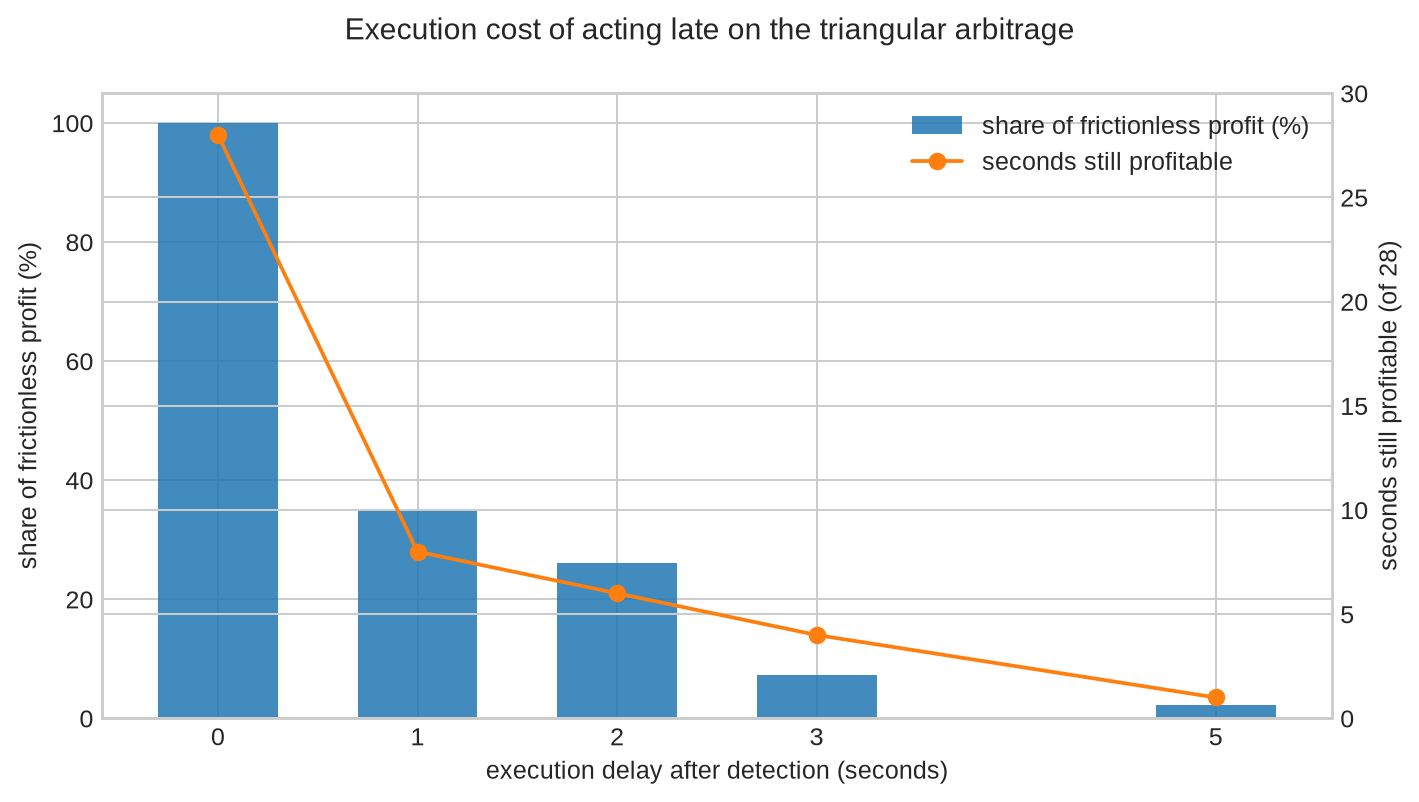
\includegraphics[width=0.8\linewidth]{outputs/figures/A2_arbitrage_execution_decay.png}
\caption{Execution cost of acting late. Each of the 28 eligible seconds is re-priced at the executable quotes and binding quantity $d$ seconds after detection, keeping the loop direction chosen at detection. Bars give the share of the frictionless \$678 that survives; the line gives the number of seconds that remain profitable.}
\label{fig:execution_decay}
\end{figure}

\begin{figure}[htbp]
\centering
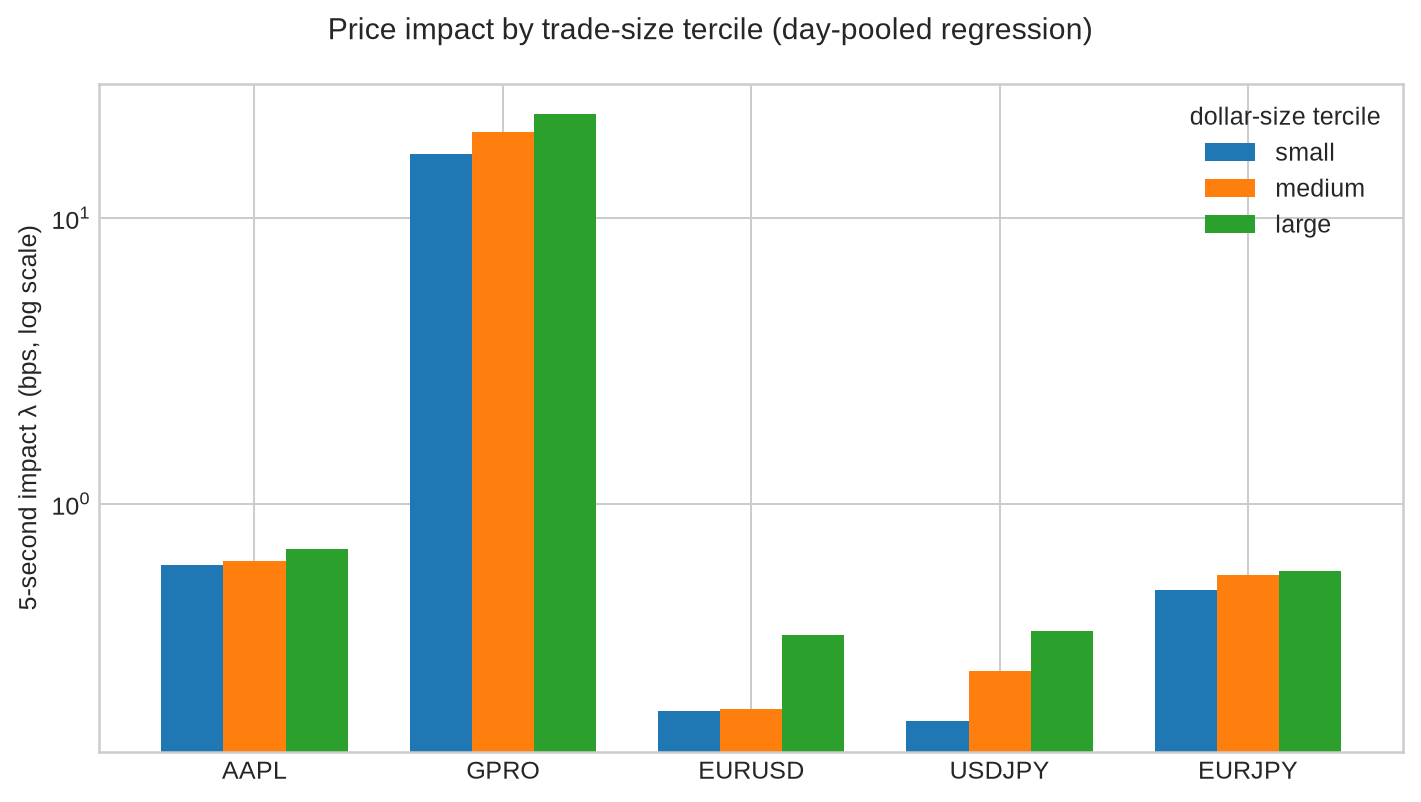
\includegraphics[width=0.8\linewidth]{outputs/figures/A3_impact_by_trade_size.png}
\caption{Five-second price impact by dollar-size tercile of the trade. The regression of equation (4) is pooled over the session and estimated within each tercile. Impact increases with trade size in every instrument; the vertical axis is logarithmic.}
\label{fig:impact_by_size}
\end{figure}
